\documentclass[10pt]{article}
\usepackage[utf8]{inputenc}
\usepackage[T1]{fontenc}
\usepackage{amsmath}
\usepackage{amsfonts}
\usepackage{amssymb}
\usepackage{mhchem}
\usepackage{stmaryrd}
\usepackage{bbold}
\usepackage{graphicx}
\usepackage[export]{adjustbox}
\graphicspath{ {./images/} }

\title{Optimal control with phase constraints for a quasilinear endovenous laser ablation model }


\author{Alexander Chebotarev, Andrey Kovtanyuk, Nikolai Park, Pavel Mesenev\\
Far Eastern Federal University, Far Eastern Center for Research and Education\\
in Mathematics, Vladivostok, Russia;\\
Institute for Applied Mathematics, FEB RAS, Vladivostok, Russia;\\
e-mail: chebotarev. ayu@dvfu.ru, kovtanyuk. ae@dvfu.ru}
\date{}


\begin{document}
\maketitle


\begin{abstract}
An optimal control problem for quasilinear equations of radiative-conductive heat transfer simulating the process of endovenous laser ablation in a bounded domain with the reflecting boundary is studied. In a given subdomain, it is required to provide a given temperature distribution, while the temperature in another given subdomain cannot exceed a critical value. On the basis of estimates of the solution of the controlled system, the solvability of the control problem is proved. An algorithm for solving the optimal control problem by minimizing the objective functional with a penalty is proposed. The efficiency of the algorithm is illustrated by a numerical example.
\end{abstract}

\section{INTRODUCTION}
The procedure of endovenous laser ablation (EVLA) is safe and sufficiently effective in the treatment of varicose veins [1]. During EVLA, a laser optical fiber is inserted into the damaged vein. Then the laser radiation is transmitted through the fiber, which at this time is pulled out of the vein. The end of the optical fiber is usually covered with a carbonized layer (optical fiber tip). The carbonized layer divides the laser energy into the optical fiber tip heating and radiation. The heat from the optical fiber tip is transferred to the blood by the conductive heat exchange, the heat transfer is significantly increased by the flow of bubbles formed at the heated fiber tip. The radiation entering the blood and surrounding tissue is partially absorbed with the release of heat. As a result, the generated thermal energy causes significant heating of the vein which leads to its obliteration (vein closure).

Mathematical modeling of radiation and thermal processes arising during EVLA is important to determine optimal parameters of radiation that provide a sufficiently high temperature inside the vein for successful obliteration, on the other hand, the generated temperature field should be relatively safe for the tissue surrounding the vein. The results of numerical simulation of EVLA for wavelengths in the range from 810 to $1470 \mathrm{~nm}$ and different vein diameters are discussed in [2-4]. In [5], the importance of mathematical modeling for choosing the optimal power of laser radiation and pullback speed of the fiber is noted. Usually, when choosing the optimal radiation parameters, the direct multiple modeling is used [2-5]. This approach is not effective in a practical point of view. Moreover, issues related to the existence and uniqueness of the optimal regime remain open.

The most promising approach to choose the optimal parameters of radiation is to consider an optimal control problem for equations of reaction-diffusion type describing the EVLA procedure. Different approaches to the analysis and parameters optimization for reaction-diffusion models describing various natural phenomena can be found in [6-9].

Optimal control problems for the model of EVLA are considered in [10,11]. In [10], an optimal control problem for the reaction-diffusion model describing the EVLA procedure is posed, which consists in approximation of a given temperature profile at a certain point of the model domain. In [11], the similar as in [10] optimal control problem is studied. Here, the objective functional is taken such that its minimization allows one to reach the given temperature distribution in different parts of the model domain. This makes it possible to provide a sufficiently high temperature inside the vein for its successful obliteration and a safe temperature in the perivenous tissue. The unique solvability of the initial-boundary value problem is proved, on the basis of which the solvability of the optimal control problem is shown. An algorithm for finding a solution of the optimal control problem is proposed. Its efficiency is illustrated by a numerical example.

In the current work, an optimal control problem for quasilinear equations of radiative-conductive heat transfer simulating the process of endovenous laser ablation in a bounded domain $\Omega$ with the reflecting boundary $\Gamma=\partial \Omega$ is considered. The problem is to minimize the functional,
$$
J(\theta)=\int_{0}^{T} \int_{G_{1}}\left(\theta-\theta_{d}\right)^{2} d x d t \rightarrow \inf
$$
on the solutions of the initial-boundary value problem:
$$
\begin{aligned}
&\sigma \partial \theta / \partial t-\operatorname{div}(k(\theta) \nabla \theta)-\beta \varphi=u_{1} \chi \\
&-\operatorname{div}(\alpha \nabla \varphi)+\beta \varphi=u_{2} \chi, \quad x \in \Omega, \quad t \in(0, T), \\
&\theta=\left.0\right|_{\Gamma}, \quad \alpha \partial_{n} \varphi+\left.2^{-1} \varphi\right|_{\Gamma}=0,\left.\quad \theta\right|_{t=0}=\theta_{0}
\end{aligned}
$$
This takes into account the restrictions:
$$
u_{1,2} \geq 0, \quad u_{1}+u_{2} \leq P,\left.\quad \theta\right|_{G_{2}} \leq \theta_{*}
$$
Here, $G_{1}$ and $G_{2}$ are subdomains of $\Omega, \theta$ is the difference between the real temperature (units in Celsius) and the constant boundary temperature, $\varphi$ is the intensity of radiation averaged over all directions, $\alpha$ is the photon diffusion coefficient, $\beta$ is the absorption coefficient, $k(\theta)$ is the coefficient of thermal conductivity, $\sigma(x, t)$ is the product of the specific heat capacity and the volume density, $u_{1}$ describes the power of the source spending on heating the fiber tip, $u_{2}$ is the power of the source spending on radiation, $P$ is the maximal power of laser source, $\chi$ is the characteristic function of the part of the medium in which the fiber tip is located divided by the volume of the fiber tip. Note that the values of the parameters $u_{1}$ and $u_{2}$ are determined by a technique of the fiber tip carbonization. An overview of some ways of the carbonization is given in $[10]$.

Thus, when modeling the EVLA procedure, we will use the diffusion model that takes into account the conductive heat transfer, as well as the radiation transfer and absorption with the release of heat. The flow of bubbles formed at the heated optical fiber tip makes a significant contribution to the temperature field. In [2-4], based on an evaluation of experimental data, the heat transfer by the flow of bubbles is modeled using a piecewise constant thermal conductivity coefficient which depends on temperature as follows: when the temperature at some point reaches $95^{\circ} \mathrm{C}$, the coefficient of thermal conductivity increases 200 times.

Following the optimal control problem, it is required to provide a given distribution of the temperature field $\theta_{d}$ in the subdomain $G_{1}$, while the temperature in the subdomain $G_{2}$ cannot exceed (if it is possible) the critical value $\theta_{*}=$ Const $>0$. 2 FORMALIZATION OF THE OPTIMAL CONTROL PROBLEM

In what follows, we assume that $\Omega$ is a Lipschitz bounded domain, $\Gamma=\partial \Omega, Q=\Omega \times(0, T)$, $\Sigma=\Gamma \times(0, T)$. We denote by $L^{p}, 1 \leq p \leq \infty$, the Lebesgue space, by $H^{1}$ the Sobolev space $W_{2}^{1}$, by $H_{0}^{1}$ a subspace of functions from $H^{1}$ with zero boundary values, and by $L^{p}(0, T ; X)$ the Lebesgue space of functions from $L^{p}$, defined on $(0, T)$, with values in Banach space $X$.

Let $H=L^{2}(\Omega), V=H_{0}^{1}(\Omega)$, and the space $V^{\prime}$ be the dual to $V$. Then we identify $H$ with its dual space $H^{\prime}$ such that $V \subset H^{1}(\Omega) \subset H=H^{\prime} \subset$ $\left(H^{1}(\Omega)\right)^{\prime} \subset V^{\prime}$, and denote by $\|\cdot\|$ the norm in $H$, and by $(h, v)$ the value of functional $h \in V^{\prime}$ on the element $v \in V$ coinciding with the inner product in $H$ if $h \in H$. The inner product in $V$ is defined as $(u, v)_{V}=(\nabla u, \nabla v)$

We assume that the following conditions hold:

(c1) $\sigma_{0} \leq \sigma \leq \sigma_{1}, \quad|\partial \sigma / \partial t| \leq \sigma_{2}$

(c2) $k_{0} \leq k(s) \leq k_{1}, \quad\left|k^{\prime}(s)\right| \leq k_{2}, \quad s \in \mathbb{R}$,

(c3) $\theta_{0} \in H$

(c4) $\alpha_{0} \leq \alpha(x) \leq \alpha_{1}, \beta_{0} \leq \beta(x) \leq \beta_{1}, \quad x \in \Omega$,

where $\sigma_{i}, k_{i}, \alpha_{i}$, and $\beta_{i}$ are positive constants.

We define a nonlinear operator $A: V \rightarrow V^{\prime}$ and linear operator $B: H^{1}(\Omega) \rightarrow\left(H^{1}(\Omega)\right)^{\prime}$ using the following equalities valid for any $\theta, v \in V, \varphi, w \in$ $H^{1}(\Omega)$
$$
\begin{aligned}
&(A(\theta), v)=(k(\theta) \nabla \theta, \nabla v)=(\nabla h(\theta), \nabla v) \\
&(B \varphi, w)=(\alpha \nabla \varphi, \nabla w)+(\beta \varphi, w)+2^{-1} \int_{\Gamma} \varphi w d \Gamma
\end{aligned}
$$
where
$$
h(s)=\int_{0}^{s} k(r) d r .
$$
Definition 1. Let $u_{1,2} \in L^{2}(0, T)$. The pair of functions $\theta \in L^{2}(0, T ; V), \varphi \in L^{2}\left(0, T ; H^{1}(\Omega)\right)$ is $a$ weak solution of the problem (1), (2) if $\sigma \theta^{\prime} \in$ $L^{2}\left(0, T ; V^{\prime}\right)$ and

$\sigma \theta^{\prime}+A(\theta)-\beta \varphi=u_{1} \chi, \quad \theta(0)=\theta_{0}, \quad B \varphi=u_{2} \chi$ where $\theta^{\prime}=d \theta / d t$.

It follows from the Lax-Milgram lemma that for any function $g \in H$ there is a unique solution of equation $B \varphi=g$. Moreover, the inverse operator $B^{-1}: H \rightarrow H^{1}(\Omega)$ is continuous. Therefore, we can exclude the radiation intensity $\varphi=u_{2} B^{-1} \chi$ and formulate the optimal control problem as follows.

\section{Problem (P)}
$$
J(\theta)=\int_{0}^{T} \int_{G_{1}}\left(\theta-\theta_{d}\right)^{2} d x d t \rightarrow \inf
$$
$$
\begin{aligned}
& \sigma \theta^{\prime}+A(\theta)=u, \quad \theta(0)=\theta_{0},\left.\quad \theta\right|_{G_{2}} \leq \theta_{*}, \quad u \in U_{a d},
\end{aligned}
$$
where
$$
\begin{array}{r}
U_{a d}=\left\{u=u_{1} \chi+u_{2} \beta B^{-1} \chi: u_{1,2} \in L^{2}(0, T),\right. \\
\left.u_{1,2} \geq 0, u_{1}+u_{2} \leq P\right\}
\end{array}
$$

\section{PRELIMINARY RESULTS}
Let us consider the problem
$$
\sigma \theta^{\prime}+A(\theta)=f, \quad \theta(0)=\theta_{0} .
$$
The following lemma is true [11].

Lemma 1. Let conditions (c1)-(c3) hold and $f \in$ $L^{2}\left(0, T ; V^{\prime}\right)$. Then there is a solution of problem (3) such that $\theta \in L^{\infty}(0, T ; H)$ and the following estimates are valid:
$$
\begin{gathered}
\|\theta(t)\|^{2} \leq \frac{K}{\sigma_{0}} \exp \frac{\sigma_{2} t}{\sigma_{0}} \quad \text { a.e. on }(0, T) \\
\int_{0}^{T}\|\theta(t)\|_{V}^{2} d t \leq \frac{K}{k_{0}}\left(1+\frac{\sigma_{2} T}{\sigma_{0}} \exp \frac{\sigma_{2} T}{\sigma_{0}}\right)
\end{gathered}
$$
where $K=\sigma_{1}\left\|\theta_{0}\right\|^{2}+k_{0}^{-1}\|f\|_{L^{2}\left(0, T ; V^{\prime}\right)}^{2}$.

The following result is important for establishing the non-emptiness of the set of admissible controlstate pairs.

Lemma 2. Let conditions (c1)-(c3) hold, $f=0$, $\theta_{0} \leq \theta_{*}$ a.e. in $\Omega$, and $\theta$ be a solution to the problem (3). Then $\theta \leq \theta_{*}$ a.e. in $\Omega \times(0, T)$.

Proof. Multiplying, in the sense of the inner product in $H$, the first equation of $(3)$ by $v=\max \{\theta-$ $\left.\theta_{*}, 0\right\} \in L^{2}(0, T ; V)$, we obtain
$$
\left(\sigma v^{\prime}, v\right)+(k(\theta) \nabla v, \nabla v)=0 .
$$
Discarding the nonnegative second term, we arrive at the estimate
$$
\frac{d}{d t}(\sigma v, v) \leq\left(\sigma_{t} v, v\right) \leq \sigma_{2}\|v\|^{2} .
$$
Taking into account that $\left.v\right|_{t=0}=0$, integrate the last inequality over time. Then
$$
\sigma_{0}\|v(t)\|^{2} \leq(\sigma v(t), v(t)) \leq \sigma_{2} \int_{0}^{t}\|v(\tau)\|^{2} d \tau
$$
Based on Gronwall's lemma, we conclude that $v=0$ and therefore $\theta \leq \theta_{*}$ a.e. in $\Omega \times(0, T)$. 4 Solvability OF THE OPTIMAL CONTROL PROBLEM

Theorem 1. Let conditions (c1)-(c3) hold, and $\theta_{0} \leq \theta_{*}$ a.e. in $\Omega$. Then a solution to the problem $(\mathrm{P})$ exists.

Proof. By Lemmas 1 and 2, the set of admissible pairs is nonempty. Let us consider a minimizing sequence of admissible pairs $\left\{\theta_{m}, u_{m}\right\} \in$ $L^{2}(0, T ; V) \times U_{a d}$ such that $J\left(\theta_{m}\right) \rightarrow j=\inf J$ where
$$
\sigma \theta_{m}^{\prime}+A\left(\theta_{m}\right)=u_{m}, \quad \theta_{m}(0)=\theta_{0},\left.\quad \theta_{m}\right|_{G_{2}} \leq \theta_{*} .
$$
The boundedness in $L^{2}(0, T ; H)$ of the set of admissible controls $U_{a d}$ implies, by Lemma 1 , the estimates:
$$
\begin{gathered}
\left\|\theta_{m}\right\|_{L^{\infty}(0, T ; H)} \leq C, \quad\left\|\theta_{m}\right\|_{L^{2}(0, T ; V)} \leq C, \\
\left\|h\left(\theta_{m}\right)\right\|_{L^{2}(0, T ; V)} \leq C .
\end{gathered}
$$
Here and below in the proof of the theorem, by $C$ we denote constants independent on $m$. The estimates (5), using if necessary subsequences, lead to the existence of functions $u \in U_{a d}, \quad \theta \in L^{2}(0, T ; V)$, $\chi \in L^{2}(0, T ; V)$ such that
$$
\begin{aligned}
& u_{m} \rightarrow u \text { weakly in } L^{2}(0, T ; H), \\
& \theta_{m} \rightarrow \theta \text { weakly in } L^{2}(0, T ; V) \text {, } \\
& \text { *-weakly in } L^{\infty}(0, T ; H) \text {, } \\
& h\left(\theta_{m}\right) \rightarrow \chi \text { weakly in } L^{2}(0, T ; V) \text {. }
\end{aligned}
$$
The convergence results (6) are sufficient for passing to the limit as $m \rightarrow \infty$ in the system (4) and proving that the limit function $\theta \in L^{2}(0, T ; V)$ is such that $\sigma \theta^{\prime} \in L^{2}\left(0, T ; V^{\prime}\right)$ satisfies the equality
$$
\left(\sigma \theta^{\prime}, v\right)+(\nabla \chi, \nabla v)=(u, v) \quad \forall v \in V
$$
and the initial condition is valid.

The following estimate guarantees the compactness of the sequence $\theta_{m}$ in $L^{2}(Q)$ :
$$
\int_{0}^{T-\delta}\left\|\theta_{m}(s+\delta)-\theta_{m}(s)\right\|^{2} d s \leq C \delta
$$
From the inequality (7), using if necessary subsequences, we obtain that $\theta_{m} \rightarrow \theta$ in $L^{2}(Q)$. Therefore, by virtue of the inequality
$$
\left|h\left(\theta_{m}\right)-h(\theta)\right| \leq k_{1}\left|\theta_{m}-\theta\right|,
$$
we conclude that $h\left(\theta_{m}\right) \rightarrow h(\theta)$ in $L^{2}(Q)$ and hence $\chi=h(\theta)$. In addition, the limit function $\theta$ satisfies the inequality $\left.\theta\right|_{G_{2}} \leq \theta_{*}$. Hence, the limit pair $\{\theta, u\} \in L^{2}(0, T ; V) \times U_{a d}$ is admissible. Since the functional $J$ is weakly lower semicontinuous,
$$
j \leq J(\theta) \leq \liminf J\left(\theta_{m}\right)=j,
$$
then the pair $\{\theta, u\}$ is a solution of the problem $(\mathrm{P})$.

\section{PENALTY PROBLEM}
To solve numerically the optimal control problem with phase constraints $\left.\theta\right|_{G_{2}} \leq \theta_{*}$, consider the following penalty problem.

$\operatorname{Problem}\left(\mathbf{P}_{\varepsilon}\right): J_{\varepsilon}(\theta) \rightarrow \inf$, where
$$
\begin{aligned}
& J_{\varepsilon}(\theta)=\int_{0}^{T} \int_{G_{1}}\left(\theta-\theta_{d}\right)^{2} d x d t \\
& +\frac{1}{\varepsilon} \int_{0}^{T} \int_{G_{2}} F(\theta) d x d t, \\
& \sigma \theta^{\prime}+A(\theta)=u, \quad \theta(0)=\theta_{0}, \quad u \in U_{a d} .
\end{aligned}
$$
Here,
$$
F(\theta)= \begin{cases}0, & \text { if } \theta \leq \theta_{*} \\ \left(\theta-\theta_{*}\right)^{2}, & \text { if } \theta>\theta_{*}\end{cases}
$$
The estimates presented in Lemma 1 also make it possible to prove the solvability of the problem with the penalty similar to the proof of Theorem 1 .

Theorem 2. Let conditions (c1)-(c3) hold. Then a solution to the problem $\left(\mathrm{P}_{\varepsilon}\right)$ exists.

Consider the approximation properties of solutions to the problem with the penalty. Let $\left\{\theta_{\varepsilon}, u_{\varepsilon}\right\}$ be solutions to problem $\left(\mathrm{P}_{\varepsilon}\right)$ and $\{\theta, u\}$ be a solution to problem $(\mathrm{P})$. Then,
$$
\sigma \theta_{\varepsilon}^{\prime}+A\left(\theta_{\varepsilon}\right)=u_{\varepsilon}, \quad \theta_{\varepsilon}(0)=\theta_{0} .
$$
Since $\left.\theta\right|_{G_{2}} \leq \theta_{*}$, the following inequality is true:
$$
\begin{array}{r}
\int_{0}^{T} \int_{G_{1}}\left(\theta_{\varepsilon}-\theta_{d}\right)^{2} d x d t+\frac{1}{\varepsilon} \int_{0}^{T} \int_{G_{2}} F\left(\theta_{\varepsilon}\right) d x d t \\
\leq \int_{0}^{T} \int_{G_{1}}\left(\theta-\theta_{d}\right)^{2} d x d t=J(\theta)
\end{array}
$$
Hence,
$$
\begin{aligned}
&\int_{0}^{T} \int_{G_{1}}\left(\theta_{\varepsilon}-\theta_{d}\right)^{2} d x d t \leq J(\theta) \\
&\int_{0}^{T} \int_{G_{2}} F\left(\theta_{\varepsilon}\right) d x d t \leq \varepsilon J(\theta)
\end{aligned}
$$
From the obtained estimates, using if necessary subsequences corresponding to $\varepsilon_{k} \rightarrow+0$, similar to the proof of Theorem 1 , we establish the existence of functions $\widehat{u} \in U_{a d}, \widehat{\theta} \in L^{2}(0, T ; V)$, such that
$$
\begin{aligned}
u_{\varepsilon} & \rightarrow \widehat{u} \text { weakly in } L^{2}(0, T ; H) \\
\theta_{\varepsilon} \rightarrow \widehat{\theta} \text { weakly in } L^{2}(0, T ; V) \\
& \text { strongly in } L^{2}(0, T ; H) .
\end{aligned}
$$
Note that
$$
\begin{aligned}
&\int_{0}^{T} \int_{G_{2}} F\left(\theta_{\varepsilon}\right) d x d t \rightarrow \int_{0}^{T} \int_{G_{2}} F(\widehat{\theta}) d x d t \\
&\int_{0}^{T} \int_{G_{2}} F\left(\theta_{\varepsilon}\right) d x d t \rightarrow 0, \text { as } \varepsilon \rightarrow+0
\end{aligned}
$$
which guarantees that $F(\widehat{\theta})=0$ and $\left.\widehat{\theta}\right|_{G_{2}} \leq \theta_{*}$.

The convergence results are sufficient for passing to the limit as $\varepsilon \rightarrow+0$ in system (8) and proving that the limit pair $\{\widehat{\theta}, \widehat{u}\} \in L^{2}(0, T ; V) \times U_{a d}$ is admissible to the problem $(\mathrm{P})$. Since the functional $J$ is weakly lower semicontinuous,
$$
j \leq J(\widehat{\theta}) \leq \liminf J\left(\theta_{\varepsilon}\right) \leq J(\theta)=j=\inf J,
$$
then the pair $\{\widehat{\theta}, \widehat{u}\}$ is a solution to the problem $(\mathrm{P})$.

Theorem 3. Let conditions (c1)-(c3) hold, and $\theta_{0} \leq \theta_{*}$ a.e. in $\Omega$. If $\left\{\theta_{\varepsilon}, u_{\varepsilon}\right\}$ are solutions to the problem $\left(\mathrm{P}_{\varepsilon}\right)$ for $\varepsilon>0$, then there is a sequence as $\varepsilon \rightarrow+0$
$$
\begin{aligned}
&u_{\varepsilon} \rightarrow \widehat{u} \text { weakly in } L^{2}(0, T ; H) \\
&\theta_{\varepsilon} \rightarrow \widehat{\theta} \text { strongly in } L^{2}(0, T ; H),
\end{aligned}
$$
where $\{\widehat{\theta}, \widehat{u}\}$ is a solution to the problem $(\mathrm{P})$.

\section{NuMERICAL ALGORITHM AND ITS IMPLEMEN- TATION}
Let us consider an iterative algorithm for solving the optimal control problem $\left(\mathrm{P}_{\varepsilon}\right)$ for the case when the control parameters $u_{1}$ and $u_{2}$ are independent of time. At each iteration of the algorithm, a linearquadratic optimal control problem is solved, in which it is required to find a minimum of the functional:
$$
\begin{aligned}
&\widehat{J}_{\varepsilon}(\theta)=\int_{0}^{T} \int_{G_{1}}\left(\theta-\theta_{d}\right)^{2} d x d t \\
&+\frac{1}{\varepsilon} \int_{0}^{T} \int_{G_{*}}\left(\theta-\theta_{*}\right)^{2} d x d t \rightarrow \inf , \quad u \in U_{a d}
\end{aligned}
$$
with restrictions
$$
\begin{aligned}
&\sigma \partial \theta / \partial t-\operatorname{div}(k(\widehat{\theta}) \nabla \theta)=u, \quad x \in \Omega, \quad 0<t<T, \\
&\left.\theta\right|_{\Gamma}=0, \quad \theta(x, 0)=\theta_{0} .
\end{aligned}
$$
Here,
$$
\begin{gathered}
U_{a d}=\left\{u=u_{1} \chi+u_{2} \beta B^{-1} \chi: u_{1,2} \in \mathbb{R},\right. \\
\left.u_{1,2} \geq 0, u_{1}+u_{2} \leq P\right\}, \\
G_{*}=\left\{x \in G_{2}: \hat{\theta}(x, t)>\theta_{*}\right\} .
\end{gathered}
$$
The function $\widehat{\theta}$ describes the temperature field found at the previous iteration.

As a dependence of the coefficient of thermal conductivity on temperature, a smooth approximation of the piecewise constant function considered in $[2-4]$ is used.

As it is easy to see, the problem (9), (10) is reduced to finding the minimum of the quadratic function of the parameters $u_{1}$ and $u_{2}$ :
$$
\widehat{J}_{\varepsilon}\left(u_{1} \Theta_{1}+u_{2} \Theta_{2}+\Theta_{3}\right) \rightarrow \inf
$$
on the triangle $\left\{u_{1}, u_{2} \in \mathbb{R}: u_{1,2} \geq 0, u_{1}+u_{2} \leq P\right\}$. The functions $\Theta_{1}, \Theta_{2}$, and $\Theta_{3}$ are calculated in advance as solutions of the following linear initialboundary value problems for $x \in \Omega, t \in(0, T)$ :
$$
\begin{aligned}
&\sigma \partial \Theta_{1} / \partial t-\operatorname{div}\left(k(\widehat{\theta}) \nabla \Theta_{1}\right)=\chi, \\
&\left.\Theta_{1}\right|_{\Gamma}=0, \quad \Theta_{1}(x, 0)=0 \\
&\sigma \partial \Theta_{2} / \partial t-\operatorname{div}\left(k(\widehat{\theta}) \nabla \Theta_{2}\right)=\beta B^{-1} \chi, \\
&\left.\Theta_{2}\right|_{\Gamma}=0, \quad \Theta_{2}(x, 0)=0 \\
&\sigma \partial \Theta_{3} / \partial t-\operatorname{div}\left(k(\widehat{\theta}) \nabla \Theta_{3}\right)=0 \\
&\left.\Theta_{3}\right|_{\Gamma}=0, \quad \Theta_{3}(x, 0)=\theta_{0} .
\end{aligned}
$$
When conducting numerical experiments, the model domain in a cylindrical coordinate system with angular symmetry as shown in Fig. 1 was used. The thickness of the carbonized layer is equal to $0.2 \mathrm{~mm}$, the pullback speed of the fiber is $2 \mathrm{~mm} / \mathrm{s}$. The radiation with wavelength of $1064 \mathrm{~nm}$ was considered. The optical and thermophysical parameters of the medium were taken from $[2-4]$.

To demonstrate the convergence of the iterative algorithm, the function $\theta_{d}$ was chosen as a solution to the direct initial-boundary value problem for $\left(u_{1}, u_{2}\right)=(3,7)$ (hereinafter units in Watts). The domains $G_{1}$ and $G_{2}$ are taken as sufficiently small neighborhoods of the points $(1.5,10),(3.5,10)$. To realize the iterative algorithm, we took $\varepsilon=0.3$ and $\theta_{*}$ corresponding to $47^{\circ} \mathrm{C}$.

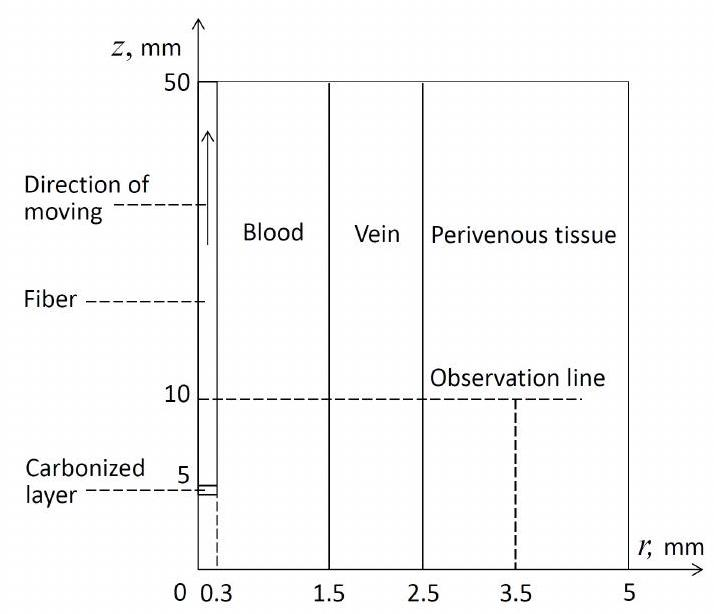
\includegraphics[max width=\textwidth]{2022_10_23_0545711a836d5ec06b12g-5}

Figure 1: Computational domain.

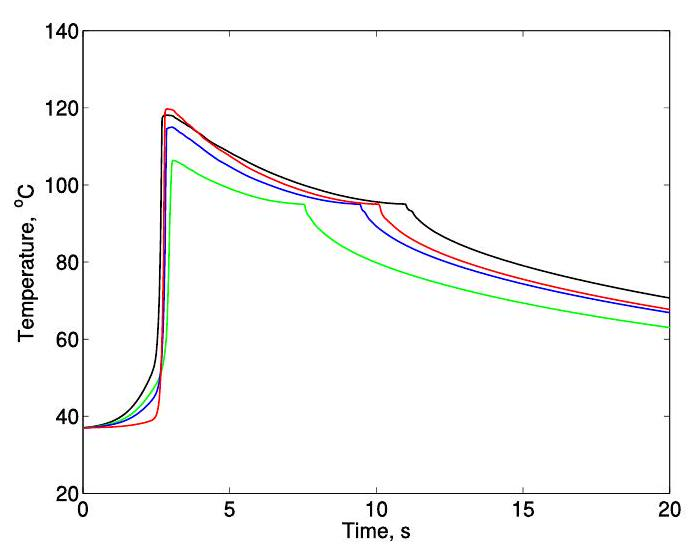
\includegraphics[max width=\textwidth]{2022_10_23_0545711a836d5ec06b12g-5(1)}

Figure 2: Temperature profiles: the desired temperature (black), 1st (green), 2nd (blue), and 3rd (red) approximations.

The approximations of the solution at the point $(1.5,10)$ is shown in Fig. 2. The approximation after 1st, 2nd, and 3rd steps of the iterative algorithm is marked in green $\left(\left(u_{1}, u_{2}\right)=\right.$ $(2.5,4.8))$, blue $\left(\left(u_{1}, u_{2}\right)=(3.4,3.5)\right)$, and red $\left(\left(u_{1}, u_{2}\right)=(4.2,0.9)\right)$, accordingly. The black line shows the desired temperature corresponding to $\left(u_{1}, u_{2}\right)=(3,7)$. The maximum value of the temperature at the point $(3.5,10)$ is $48.8^{\circ} \mathrm{C}$. Note that, when $\left(u_{1}, u_{2}\right)=(3,7)$, the maximum value of the temperature at the point $(3.5,10)$ is equal to $50.2^{\circ} \mathrm{C}$.

The experiment demonstrates an opportunity for reducing the temperature in the perivenous tissue while maintaining the temperature regime inside the vein.

\section{ACKNOWLEDGEMENTS}
This work was supported by the Russian Foundation for Basic Research (project № 20-01-00113a) and by the Ministry of Science and Higher Education of the Russian Federation (agreement № 07502-2021-1395).

\section{REFERENCES}
[1] van den Bos, R. R., Neumann, M., de Roos, K.-P., Nijsten, T., 2009, Endovenous laser ablation-induced complications: Review of the literature and new cases, Dermatol. Surg., Vol. 35(8), pp. 1206-1214.

[2] van Ruijven, P. W. M., Poluektova, A. A., van Gemert, M. J. C., Neumann, H. A. M., Nijsten, T., van der Geld, C. W. M., 2014, Opticalthermal mathematical model for endovenous laser ablation of varicose veins, Lasers Med. Sci., Vol. 29, pp. 431-439.

[3] Poluektova, A. A., Malskat, W.S. J., van Gemert, M. J. C., Vuylsteke, M. E., Bruijninckx, C. M. A., Neumann, H. A. M., van der Geld, C. W. M., 2014, Some controversies in endovenous laser ablation of varicose veins addressed by optical-thermal mathematical modeling, Lasers Med. Sci., Vol. 29, pp. 441452.

[4] Malskat, W. S. J., Poluektova, A. A., van der Geld, C. W. M., Neumann, H. A. M., Weiss, R.A., Bruijninckx, C.M.A., van Gemert, M. J. C., 2014, Endovenous laser ablation (EVLA): A review of mechanisms, modeling outcomes, and issues for debate, Lasers Med. Sci., Vol. 29, pp. 393-403. [5] Mordon, S., Wassmer, B., Zemmouri, J., 2006, Mathematical modeling of endovenous laser treatment (ELT), BioMed. Eng. OnLine., Vol. 5, n.a. 26.

[6] Alekseev, G. V., Brizitskii, R. V., Saritskaya, Zh. Yu., 2016, Stability estimates of extremum problem's solutions for nonlinear convectiondiffusion-reaction equation, Sib. J. Industrial Math., Vol. 10, pp. 155-167.

[7] Brizitskii, R. V., Saritskaya, Zh. Yu., 2018, Optimization analysis of the inverse coefficient problem for the nonlinear convection-diffusionreaction equation, J. Inv. Ill-Posed Probl., Vol. 9, pp. 821-834.

[8] Chebotarev, A. Y., Grenkin, G. V., Kovtanyuk, A. E., Botkin, N. D., Hoffmann, K.-H., 2018 , Inverse problem with finite overdetermination for steady-state equations of radiative heat exchange, J. Math. Anal. Appl., Vol. 460, pp. $737-744$.

[9] Maslovskaya, A. G., Moroz, L. I., Chebotarev, A. Y., Kovtanyuk, A. E., 2021, Theoretical and numerical analysis of the Landau-Khalatnikov model of ferroelectric hysteresis, Commun. Nonlinear Sci. Numer. Simul., Vol. 93, n.a. 105524 .

[10] Kovtanyuk, A. E., Chebotarev, A. Yu., Astrakhantseva, A. A., Sushchenko, A. A., 2020, Optimal control of endovenous laser ablation, Opt. Spectrosc., Vol. 128(9), pp. 1508-1516.

[11] Kovtanyuk, A., Chebotarev, A., Astrakhantseva, A., 2021, Inverse extremum problem for a model of endovenous laser ablation, J. Inv. Ill-Posed Probl., Vol. 29(3), pp. 467-476.


\end{document}